%
%   Copyright 2013 Katarzyna Szawan <kat.szwn@gmail.com>
%       and Michał Rus <m@michalrus.com>
%
%   Licensed under the Apache License, Version 2.0 (the "License");
%   you may not use this file except in compliance with the License.
%   You may obtain a copy of the License at
%
%       http://www.apache.org/licenses/LICENSE-2.0
%
%   Unless required by applicable law or agreed to in writing, software
%   distributed under the License is distributed on an "AS IS" BASIS,
%   WITHOUT WARRANTIES OR CONDITIONS OF ANY KIND, either express or implied.
%   See the License for the specific language governing permissions and
%   limitations under the License.
%

\section{Scala}
\label{sec:scala}

Our language of choice for this system (for both client- and server-side) is Scala: a multi-paradigm, object-functional programming language. It compiles to Java bytecode, so it offers full compatibility with Android SDK, at the same time making the code unmeasureably more elegant and robust~\cite{Odersky:2008:Programming}.

\section{Akka.io for server-side}
\label{sec:akka}

Akka is an actor model for Scala (and Java) languages: `a toolkit and runtime for building highly concurrent, distributed, and fault tolerant event-driven applications on the JVM'~\cite{Akka:2013:Docs}. Actor model is a higher-level abstraction of concurrent programming. All operations are performed in a non-blocking fashion. Any number of servers can form one (or more) big actor cluster. Each actor is a very lightweight event-driven process; this makes it possible to create approximately 2.7 million actors per 1 GB of heap memory~\cite{Akka:2013:Docs}.

Actors can be thought of as concurrent processes which communicate by passing messages. At the same time they are really efficient: especially 1 actor is \emph{not} equivalent to 1 thread, and \emph{not even 1} lightweight JVM thread.

\section{Spray.io}
\label{sec:theory-spray}

Spray.io is a highly performant HTTP connectivity layer for Akka actors, see \cref{fig:spray-benchmark}. It also provides a convenient---and user-extendable---way of marshalling and unmarshalling of JSON requests and responses.

\begin{figure}[h]
	\centering
	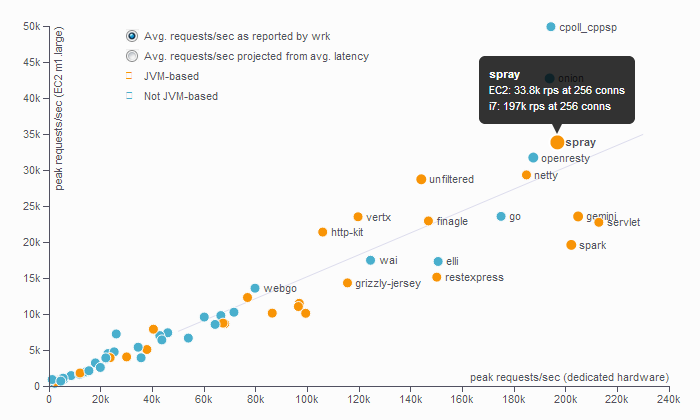
\includegraphics[width=\textwidth]{graphics-spray-benchmark}
	\caption{Benchmark of HTTP throughput of various existing solutions published by \href{http://www.techempower.com}{techempower.com} \cite{Spray:2013:Benchmark}.}
	\label{fig:spray-benchmark}
\end{figure}
